% Two maps of Congress: paper V1 (Martin, with Claude), 24 Nov 2026.
% Written to the brief in BRIEF.md: one story ("the record decides"), six pages, three figures, every choice defended
% inline. Numbers come from the result files named in the comments; none is from memory.
% To use in Overleaf: open the PNAS template, replace its main file with this one, and upload figures/ and
% references.bib from this folder. pnas-new.cls comes with the template.
\documentclass[9pt,twocolumn,twoside]{pnas-new}
\templatetype{pnasresearcharticle}
% Let the tall figures (Fig. 1 is 14.2 cm, Fig. 3 15 cm) sit at the top of a text page instead of on float pages.
\renewcommand{\topfraction}{0.9}\renewcommand{\dbltopfraction}{0.9}\renewcommand{\textfraction}{0.07}
\renewcommand{\floatpagefraction}{0.85}\renewcommand{\dblfloatpagefraction}{0.85}

\title{How divided the House looks depends on the record: names on the floor against partners on bills}

\author[a]{Anas Mir}
\author[a]{Martin M{\o}llenhus}
\author[a]{Diego A. Mijares}
\affil[a]{Technical University of Denmark, 02805 Social Graphs and Interactions}

\leadauthor{Mir}

% 2-3 sentences for a reader outside the field (course); at most 120 words (PNAS).
\significancestatement{Claims that Congress is polarized rest on whichever record is measured, most often votes or
bill sponsorship. We read three records of the same members: whom they work with on bills, whom they name in floor
debate, and whom they name to voters. Each gives a different degree of division, shaped by the rules and the
audience of the record, so a single record should not be read as the state of a legislature.}

\authorcontributions{M.M. built the shared name matcher, the floor and working maps, the null models and the
community and committee analysis, tested which bills members announce, made Figure 1, and wrote the network Results
and Methods. A.M. collected the 55,023 press releases, matched them to members and bills, measured district lean,
ran the test of exposed against safe seats and its checks, made Figure 3, and wrote the press Results and Methods.
D.A.M. measured the matcher's precision, wrote the labelling rules, coded all 100 labelled mentions, built the text
classifier, checked the speaker attribution, compiled the literature, made Figure 2, and wrote the labelling Results
and Methods. M.M. and A.M. second-coded 25 mentions each. D.A.M. and M.M. wrote the Introduction and Discussion. An
AI assistant wrote code and drafted text under the authors' direction (AI\_METHODS.md).}
\authordeclaration{The authors declare no competing interest.}
\correspondingauthor{}

\keywords{Congress $|$ polarization $|$ networks $|$ named entities $|$ null models}

% 150 words (course rule). Written last.
\begin{abstract}
Congress is usually called divided on the evidence of votes, words or cosponsorship. We ask how much that picture
depends on the record read. For the same 450 members of the 119th US House (2025--26), we build a working map
of who cosponsors whose bills and a floor map of who names whom in floor speech, found by a name matcher right in
98 of 100 hand-checked cases. At equal size, 38.7\% of floor ties cross the party line against 28.6\% of working
ties, and floor communities follow committees, not parties. The floor's rules account for about two thirds of
its party division, and of 75 cross-party mentions read by hand, 69\% give credit and 7\% criticize. In 55,023
press releases, members in close seats name the other party more often, a gap we cannot separate from ideology.
How divided the House looks depends on which record is read.
\end{abstract}

\dates{Hand-in 27 November 2026.}

\begin{document}

\maketitle
\thispagestyle{firststyle}
\ifthenelse{\boolean{shortarticle}}{\ifthenelse{\boolean{singlecolumn}}{\abscontentformatted}{\abscontent}}{}

% ============================================================================ INTRODUCTION
\dropcap{T}he US Congress is usually described as two camps, and most measurements agree. Members of the two
parties vote apart and have spoken increasingly different languages since the early 1990s \cite{gentzkow2019}.
Networks of who cosponsors whose bills \cite{fowler2006} show the same split, with ties between the parties growing
rarer over four decades \cite{neal2020}.

How deep the split looks depends, however, on the record. Between 1973 and 2004, agreement between the parties fell
in roll-call votes while staying far more stable in cosponsorship, because party leaders chose which bills reached
a vote \cite{harbridge2015}. Across channels of communication the parties are always distinguishable, but more so
in front of national audiences than local ones \cite{green2024}. Each record is produced under its own rules and
for its own audience, so division is a property of the record as well as of the members.

We add a record that can be compared with cosponsorship on equal terms: the colleagues members name. A name in a
floor speech or a press release points at one specific member, so names form a network on exactly the members of
the cosponsorship network, and the same measures and null models apply to both. Names are also harder to empty of
meaning than labels: the word ``bipartisan'' in floor speech is mostly attached to bills with token support from the
other party \cite{westwood2022}, but a named colleague can be checked against the legislative record. And members
have reasons to manage whom they show: voters with weak party ties reward a bipartisan image \cite{harbridge2011},
and what members tell constituents is a chosen presentation of their work \cite{grimmer2013}.

We therefore ask how divided the same House looks in three records: whom members work with on bills, whom they name
in floor debate, and whom they name to voters in press releases. The answer is not obvious. Members might attack
the other side in public and cooperate quietly, which would make the floor more divided than the bills, or display
the cross-party partners they have, which would make it less. We find that the floor is less divided than the bills
at equal size, that much of the difference comes from how floor debate is organized, and that the cross-party names
are mostly credit; at home, members in close seats show the other party more often.

% Figure 1 is defined here so that it lands at the top of page 2 (a full-width float appears at the earliest on
% the page after the one it is defined on).
\begin{figure*}[t]
\centering
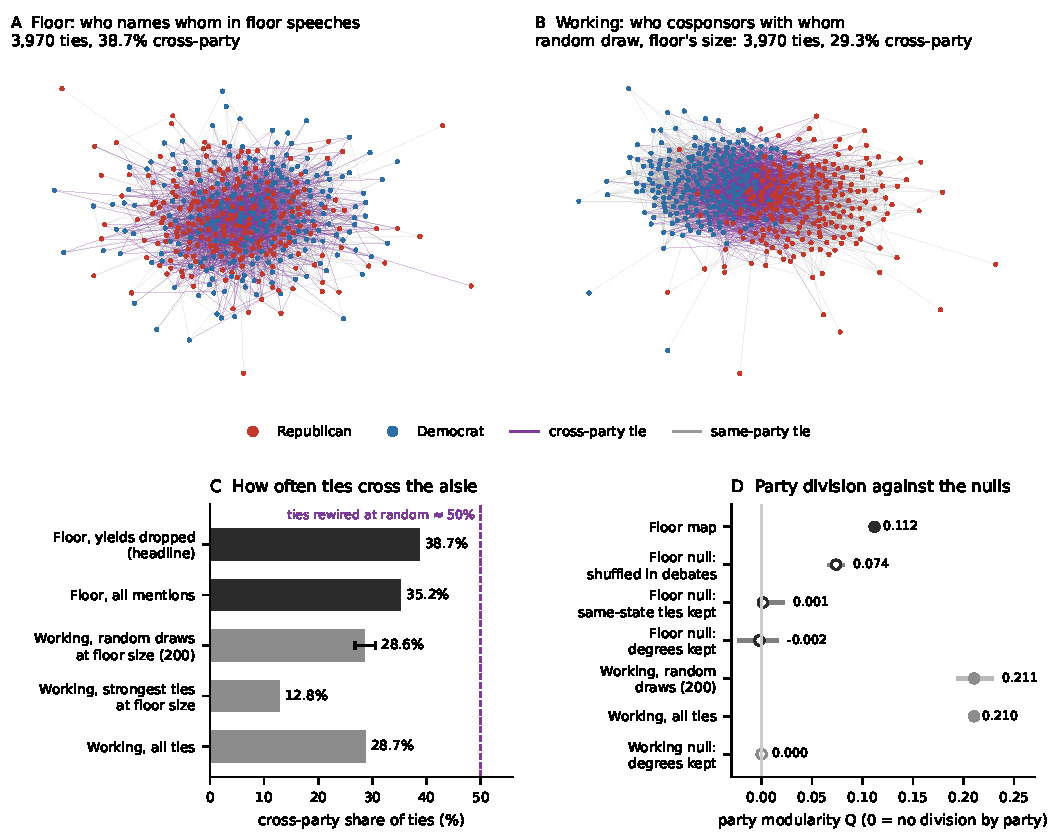
\includegraphics[width=17.8cm]{figures/figure1.pdf}
\caption{The same House as two networks, January 2025 to November 2026. (\emph{A}) Floor map: members tied when
one names the other in a floor speech, yields of debate time left out. (\emph{B}) Working map: one random draw of
sponsor--cosponsor ties, thinned to the floor map's 3,970 ties. Nodes are members (red Republican, blue Democrat);
purple ties cross the aisle; positions carry no meaning. (\emph{C}) Share of ties that cross the aisle; the bar
for the random draws shows the range over 200 draws, and the dashed line the level if ties were rewired at random.
(\emph{D}) Party modularity of each map (filled) against its nulls (open; lines show the range over the draws):
names shuffled within each debate, same-state ties kept, and each member's number of ties kept. The floor map is
less divided than the working map at equal size, and debate procedure accounts for about two thirds of its own
division.}
\label{fig:maps}
\end{figure*}

% ============================================================================ RESULTS
\section*{Results}

\subsection*{The floor map is less divided than the working map}
We built two networks on the same 450 Republicans and Democrats (Methods). In the \emph{working map}, two members
are tied if one cosponsored a bill or joint resolution that the other sponsored: a public commitment to a
colleague's bill, which misses cooperation that leaves no signature and costs little to give (46,513 ties). In the
\emph{floor map}, two members are tied if one named the other in a floor speech, leaving out the procedural naming
that hands over debate time: it captures whom members choose, or are required, to mention in public, and misses
both tone and how often (3,970 ties from 8,469 mentions).
% m3_table.csv

On the floor, 38.7\% of ties cross the aisle (Fig.~\ref{fig:maps}\emph{A},\emph{C}). Because the working map is about
twelve times denser, we compare it at equal size: in 200 random draws of 3,970 working ties, 28.6\% cross the aisle
(range 26.8\% to 30.6\%), and no draw comes within eight points of the floor (Fig.~\ref{fig:maps}\emph{B},\emph{C}).
Party modularity, which measures how strongly the party split groups the ties but not why, agrees: 0.112 on the
floor against 0.211 (0.193 to 0.230) for the draws (Fig.~\ref{fig:maps}\emph{D}). The gap does not depend on
leaving out yields of time (35.2\% against 28.7\% with them kept). Members' strongest partnerships are more partisan
still: of the 3,970 pairs who share the most bills, 12.8\% cross the aisle. Both maps are more divided than chance:
rewired with every member's number of ties kept, about half of the ties would cross and modularity would be near
zero (Fig.~\ref{fig:maps}\emph{C},\emph{D}).
% m3_table.csv, m3_random_draws.csv


\subsection*{The floor's rules shape its division}
The floor is not a free choice of whom to mention. Each debate has a cast, often a manager from each party for the
committee that wrote the bill, so members of both parties are named in the same debates by design. To measure how
much of the floor map's party division that structure explains, we shuffled who is named within each debate,
keeping who speaks and who is named in it. Modularity falls to 0.074 (0.065 to 0.082 over 200 shuffles) against
0.112 observed: the debates account for about two thirds of the division, and the rest, members naming their own
side beyond what the debate forces, exceeds every shuffle (Fig.~\ref{fig:maps}\emph{D}). State delegations
explain almost none of it: keeping each member's number of same-state ties gives a modularity of 0.001.
% m4_results.csv, m3b_state_null.csv

Communities show what the floor is organized by instead. On the working map, Louvain's communities are the two
parties (normalized mutual information with party, NMI, 0.83). On the floor map they cut across party (NMI 0.03,
against 0.29 for working draws of the same size): eight communities of 28 to 80 members, each holding both
parties. In seven of them one House committee is 3.0 to 7.9 times as common as in the House, among them
Appropriations (82\% of the community's members) and Ways and Means (79\%); the eighth gathers the party leaders.
Of all floor ties, 44\% join two members of the same committee, against 17.1\% when ties are rewired, and so do
50\% of cross-party floor ties. In the working map the share barely exceeds chance (22\% against 18.7\%). The floor
record is in large part the committee system at work in public, and that is a reason it looks less divided.
% m5_table.csv, m5_committees/committee_table.csv

\subsection*{Cross-party names on the floor are mostly credit}
A name says nothing about its tone, and a member can name the other side to attack it. We read 100 floor mentions
drawn at random, 75 between parties and 25 within, with the parties hidden from the coders, and coded what the
speaker did towards the named member (Methods). Of the cross-party mentions, 69\% (95\% interval 58\% to 79\%)
agreed with the named member: thanks to a bill's co-lead or a committee's chair, praise for joint work, support for
their bill. 23\% (15\% to 33\%) were neutral references and 7\% (3\% to 15\%) disagreed
(Fig.~\ref{fig:labels}). Two human coders agreed on 82\% of the mentions (Cohen's $\kappa = 0.64$). A text
classifier trained on these labels did not beat always answering ``agreeing'' (73\% against 72\% in leave-one-out),
so we report the hand-read shares only. These labels capture what a speaker does towards a colleague in one
sentence; they do not show that the two cooperate.
% Diego/d2_labelling/RESULTS.md, Diego/d5_classifier/results.txt

\begin{figure}[tbp]
\centering
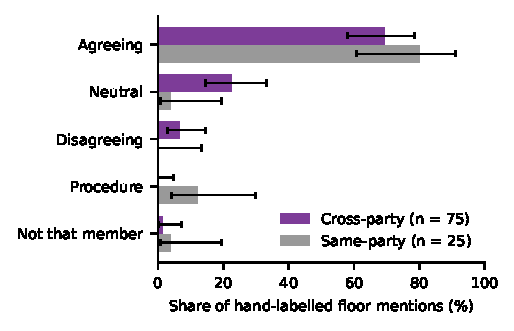
\includegraphics[width=8.7cm]{figures/figure2.pdf}
\caption{What floor mentions do. Share of 100 hand-labelled mentions in each code, for mentions between parties
(purple, $n = 75$) and within a party (grey, $n = 25$). Lines show 95\% Wilson intervals. A mention was coded ``not
that member'' when the matched name referred to someone else. Cross-party mentions are mostly agreeing and rarely
disagreeing; handing over debate time occurs only within a party.}
\label{fig:labels}
\end{figure}

\subsection*{A third record: whom members name at home}
Press releases are written for voters, not for the chamber. We cannot put them on Figure~\ref{fig:maps}'s scale:
a member's releases name few colleagues, so we ask a different question of this record, namely which members show
the other party to their voters. The measure is the share of a member's releases that name a House member of the
other party who is neither a party leader nor a co-lead of a bill the release cites; it captures whom a member
chooses to show, and misses why. A seat is \emph{exposed} when the district a member served leans toward their own
party by five points or less.
% Anas/a4/out/results.csv

Exposed members name the other party more often, in both parties (Fig.~\ref{fig:home}): exposed Republicans in
13.3\% of their releases against 9.2\% for safe Republicans, exposed Democrats in 11.6\% against 9.0\% (406 members,
53,664 releases; $p = 0.004$ for each, labels shuffled within party). The two gaps do not differ ($p = 0.36$).
Every check fixed before the analysis keeps both gaps positive (Fig.~\ref{fig:home}\emph{B}), and three blind AI
readers found that 46 of 60 counted names (77\%) named a partner or praised the member and one criticized. But
exposed members are also their party's moderates, and among members of similar ideology little of the gap remains
(1.1 of 4.1 points for Republicans, 0.2 of 2.6 for Democrats; $p = 0.39$ and $0.76$): the data cannot say whether
the seat or the member's ideology drives the naming.
% Anas/a4/out/results.csv, a4/check_tone/scored.csv, a4/out/ideology_check.csv

The bills members show follow a milder version of the same pattern. Of a member's own bills, those with an
original cosponsor of the other party were cited in their releases more often than the rest (52.7\% against 45.1\%;
388 members, 10,125 bills; $p < 0.001$ against a shuffle within each member), but most of that gap separates co-led
bills from solo bills: against bills co-led by their own party only, the difference is 3.5 points ($p = 0.02$).
% Martin/m6_results.csv

\begin{figure}[tbp]
\centering
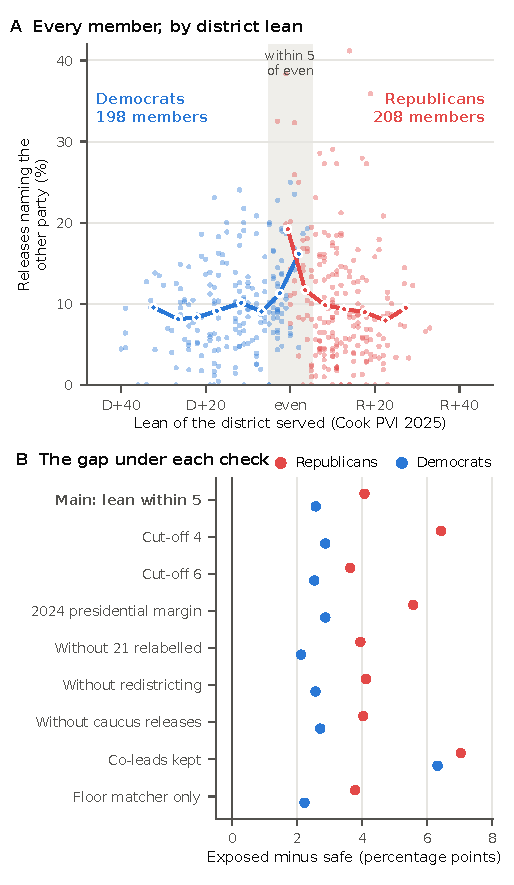
\includegraphics[width=8.7cm]{figures/figure3.pdf}
\caption{Members in exposed seats name the other party more often in their press releases. (\emph{A}) Each dot is
one of 406 members (53,664 releases, January 2025 to November 2026): the share of their releases naming a House
member of the other party who is neither a party leader nor a co-lead of a cited bill, against the lean of the
district they served (Cook PVI 2025). Lines join band means; shading marks seats within five points of even.
(\emph{B}) Exposed minus safe mean share, by party, for the main definition and for each check fixed before the
analysis (other cut-offs, a second lean source, leaving out redrawn districts, leaving out redistricting and caucus
releases, counting co-leads, the floor's matcher alone). Every gap is positive with $p < 0.05$ (labels shuffled
within party, 10,000 shuffles).}
\label{fig:home}
\end{figure}

% ============================================================================ DISCUSSION
\section*{Discussion}
The same members, over the same two years, look different in different records. In the bills they sign together,
the House is two camps; in the colleagues they name on the floor, it is less divided, and its communities are
committees. That difference is not noise around one true level of division. The floor record is produced by
debates in which committee managers from both parties name each other, and those rules account for about two
thirds of the floor map's party division. What remains is mostly credit: members thank and praise colleagues
across the aisle far more often than they criticize them. In the third record, written for voters, members in
close seats show the other party more often.

The result does not show that members cooperate more than cosponsorship suggests. A name is a reference, not a
partnership, and the floor's procedure brings members of both parties into the same debates whether or not they
work together. The comparison also depends on how the dense working map is made comparable: against random ties
of the same number the gap is ten points, against members' strongest partnerships more than twenty-five. We report
random ties as the like-for-like comparison, because a floor tie means only ``named at least once''. At home, the
gap between exposed and safe seats may be the seat or the member: exposed members are also moderates, and we
cannot separate the two, although holding ideology fixed may also remove part of a real seat effect, since votes
in a close seat may be moderate for that reason.

Several limits are our own findings. The matcher was right in 98 of 100 hand-checked mentions and found 12 of the
13 members a reader found in 30 full turns, so recall rests on few names (95\% interval 67\% to 99\%). Its errors
are not neutral: a namesake mistaken for a member belongs to the other party about half the time, so errors push
the floor map towards looking less divided, though at 98\% precision the effect on the headline is small. The
floor map is unweighted, so a pair named once counts like a pair named fifty times. One hundred labels give wide
intervals and too few disagreements for a classifier to learn from, and coders often know a member's party even
when it is hidden. Committee lists are today's, not the start of the term. Speaker attribution held in all 60
turns we checked.

Westwood found that the word ``bipartisan'' says little about votes \cite{westwood2022}; the colleagues members
name across the aisle point instead to specific bills and committees. One Congress and one chamber cannot say
whether these patterns are stable, but the same records exist for every Congress since the Record went online. With
reliable labels for every mention, the floor map could be signed, positive for credit and negative for criticism,
and tested for whether the House splits into two camps that praise inward and criticize outward.

% ============================================================================ METHODS
\section*{Materials and Methods}

\textbf{Data.} Members are the 450 Republicans and Democrats who served in the 119th House, identified by Bioguide
ID (Voteview, with the congress-legislators project for names). Floor speech is the Congressional Record (govinfo),
6 January 2025 to 9 November 2026, downloaded 11 November 2026 and split into speaker turns; we keep the 17,824
House turns of at least 50 words spoken by a member. Speaker attribution was checked by hand on 60 random turns:
all 60 were assigned to the member the Record names as speaker (95\% Wilson interval \cite{wilson1927} 94\% to
100\%). Bills and cosponsorships come from govinfo's BILLSTATUS data for the same Congress. Press releases are
those members posted on their house.gov sites from 3 January 2025 to the download on 20 November 2026: 55,023
releases from 412 members. Not collected: four sites that load their listing only with JavaScript, one listing that
ends in 2024, and the 12 members who had left office.

\textbf{Finding names.} We extract members from text with a rule-based entity matcher, because names in the Record
follow a few fixed forms and a rule can be checked line by line. It finds a House title followed by a surname
(``Mr.\ Cole'', ``Chairman Cole''), names in a list after a plural title, and, in floor speech, full names without a
title (``my friend Chip Roy''). Shared surnames are settled by first name or nickname and then by a state name
within 80 characters; otherwise the name is dropped rather than guessed (828 titled names). Names after ``Senator'',
``Governor'' and similar titles are skipped, and members naming themselves are not counted. On 100 hand-labelled
mentions, 98 named the right member; untitled names and list names, added later, were right in 30 of 30 and 20 of
20. In 30 random turns read in full, the matcher found 12 of the 13 members a reader found (recall 92\%; the miss
was an unresolved shared surname). Press releases use the same matcher with a press layer (first names members
use in their own releases, and party--state tags such as ``R-NY''); on 40 releases read by five blind AI readers and
checked by an author, its recall was 0.97 and precision 0.96.

\textbf{Yields.} When a floor manager hands over debate time (``I yield 2 minutes to the gentleman from Texas''),
the name is procedure, not a choice to name someone, so yields are left out of the floor map. A mention is a yield
when ``yield'' (not ``yield back'') precedes the name in the same sentence, or ``for yielding'' follows it. Where this
rule and a simpler 60-character window disagreed, all 15 mentions only our rule flagged were yields, and 14 of the
15 only the window flagged were not. Keeping yields changes the gap from 10.1 to 6.5 points.

\textbf{Maps and thinning.} Both maps are undirected and unweighted, because a floor tie can only mean ``named at
least once''. Floor: two members are tied if either named the other (3,970 ties). Working: two members are tied if
one cosponsored a bill or joint resolution the other sponsored, withdrawn cosponsorships removed (46,513 ties). We
thin the working map to the floor map's size by drawing ties at random, 200 times, because random thinning changes
only the density (party modularity 0.211 on average over the draws, against 0.210 for all ties), whereas keeping
the strongest ties also changes which ties are kept (0.301). The strongest ties (pairs sharing the most bills) are reported as a separate comparison.

\textbf{Division and nulls.} Division by party is the share of ties that cross the aisle and the modularity of the
party split \cite{newman2006}. Each map is compared with three nulls, seed 2805 throughout: (i) degree-preserving
rewiring by double-edge swaps \cite{maslov2002}, five swaps per tie, 200 rewirings, because members with many ties
would cross the aisle more by chance alone; (ii) for the floor map, a shuffle of who is named within each debate
(one Record item; 200 shuffles), because debates fix who is in the room; and (iii) a rewiring that also keeps each
member's number of ties within their own state, because members name their state delegation.

\textbf{Communities.} We use the Louvain method \cite{blondel2008} (resolution 1; 50 random starts, keeping the
partition with the highest modularity, because single runs differ) and compare partitions with party, and between
maps, by normalized mutual information \cite{danon2005}. Committee membership comes from the congress-legislators
project (downloaded 22 November 2026); we count floor ties that join two members of the same full committee against
the same degree-preserving rewiring.

\textbf{Hand labels and classifier.} We drew 100 floor mentions with a fixed seed, 75 between parties and 25 within.
Coders saw the speaker, the named member, the date and three sentences of context, not the parties, and gave one
of five codes fixed in advance with rules for mixed cases: procedure, agreeing, disagreeing, neutral, or not that
member. One author coded all 100; the other two coded 25 each, and an AI coder the other 50 under the same rules
without seeing any human code. Human agreement was 82\% (Cohen's $\kappa = 0.64$ \cite{cohen1960}); the AI coder
agreed with the first coder on 88\% ($\kappa = 0.72$). Shares are the first coder's with 95\% Wilson intervals. The
classifier was a logistic regression on TF-IDF features of words and word pairs, with the named member's surname
masked, tested by leave-one-out against always predicting the most common code.

\textbf{Press releases and exposure.} District lean is the 2025 Cook PVI \cite{cook2025pvi} of the district each
member served, read from a dated Wikipedia revision \cite{wikipedia2025pvi}; it agrees with the 2024 presidential
margin \cite{downballot2024} ($r = 0.999$). We use the district served, because the releases were written for its
voters; nine states redrew their maps for 2026. The test uses the 406 members with at least ten releases. Gaps are
tested by shuffling the exposed label among members of the same party (10,000 shuffles, two-sided), because the
parties differ in size and in how often they name each other. Tone was checked on 60 counted names (15 per party and
seat, seed 2805) by three blind AI readers who did not see the seat; they agreed on 56, and an author read the other
four. For ideology, members were ranked into five bands within party by DW-NOMINATE (Voteview), and the exposed label
was shuffled only within party and band. For the bills members announce, a member's own bills are the H.R.\ and
H.J.Res.\ they sponsored, a bill is cross-party when it has an original cosponsor of the other party, a release
cites a bill by its number or a title unique to it (30 of 30 correct), and the cross-party label is shuffled among
each member's own bills (10,000 shuffles).

\textbf{AI use, data and code.} Code and drafts of the text were written with an AI assistant (Claude, Anthropic);
every place a model touched a result, and how it was checked, is listed in AI\_METHODS.md. Code, derived data and
the hand-check sheets are at \url{https://github.com/martinmoll/SocialGraphsAndInteractions}.

\bibliography{references}

\end{document}
